\documentclass[12pt]{article}
\setlength{\oddsidemargin}{0in}
\setlength{\evensidemargin}{0in}
\setlength{\textwidth}{6.5in}
\setlength{\parindent}{0in}
% \setlength{\parskip}{\baselineskip}
\usepackage{graphicx}
\usepackage{multirow}
\usepackage{multicol}
\usepackage{listings}
\usepackage{color}

\definecolor{dkgreen}{rgb}{0,0.6,0}
\definecolor{gray}{rgb}{0.5,0.5,0.5}
\definecolor{mauve}{rgb}{0.58,0,0.82}

\lstset{frame=tb,
  language=MATLAB,
  aboveskip=3mm,
  belowskip=3mm,
  showstringspaces=false,
  columns=flexible,
  basicstyle={\small\ttfamily},
  numbers=none,
  numberstyle=\tiny\color{gray},
  keywordstyle=\color{blue},
  commentstyle=\color{dkgreen},
  stringstyle=\color{mauve},
  breaklines=true,
  breakatwhitespace=true,
  tabsize=3
}

\usepackage{amsmath,amssymb,amsrefs}

\usepackage[top=24mm, bottom=18mm, left=15mm, right=13mm]{geometry}
\usepackage{url}

\title{Project 1 Report}
\author{Lawrence Ouyang}

\begin{document}
\maketitle
\section{User Guide}
Included with this project are the following four MATLAB files:
\begin{itemize}
\item Project1.m
\item AnalyticSol.m
\item MatrixRK4.m 
\item Adams4PC.m
\end{itemize}

\underline{\textit{Project1.m}} contains the steps to creating the solutions using the 2 derived methods. This script will also generate the 6 log plots. Locations of the output are explained in the comments of the script.\\ \\

\underline{\textit{AnalyticSol.m}} is the function that calculates the exact solution:
\begin{center}
$y(t) = Ve^{Dt}V^{-1}y(0) $
\end{center}
for some time $t$. Although arbitrary, the input of this function matches our other methods for consistency. It's inputs are the interval $[a,b]$, the time-step $h$, the initial value $y(0)$, and the matrix $A$. The output of this function is a vector $y$ that is the exact solution for the system of equations.\\ \\

\underline{\textit{MatrixRK4.m}} is the function that uses the RK4 method to approximate a solution for the equation:
\begin{center}
$y'(t) = Ay(t) $
\end{center}
It's inputs are the interval $[a,b]$, the time-step $h$, the initial value $y(0)$, and the matrix $A$. The outputs of this function is the approximate solution vector $y$ and the root mean square error. \\ \\

\underline{\textit{Adams4PC.m}} is the function that uses the Adams 4th Order Predictor-Corrector method to approximate a solution for the equation:
\begin{center}
$y'(t) = Ay(t) $
\end{center}
It's inputs are the interval $[a,b]$, the time-step $h$, the initial value $y(0)$, and the matrix $A$. The outputs of this function is the approximate solution vector $y$ and the root mean square error. This function uses RK4 to approximate the first 3 approximations.\\ \\

\section{Solutions}
The plots of the 2 methods and 3 sets are shown below:
\begin{center}
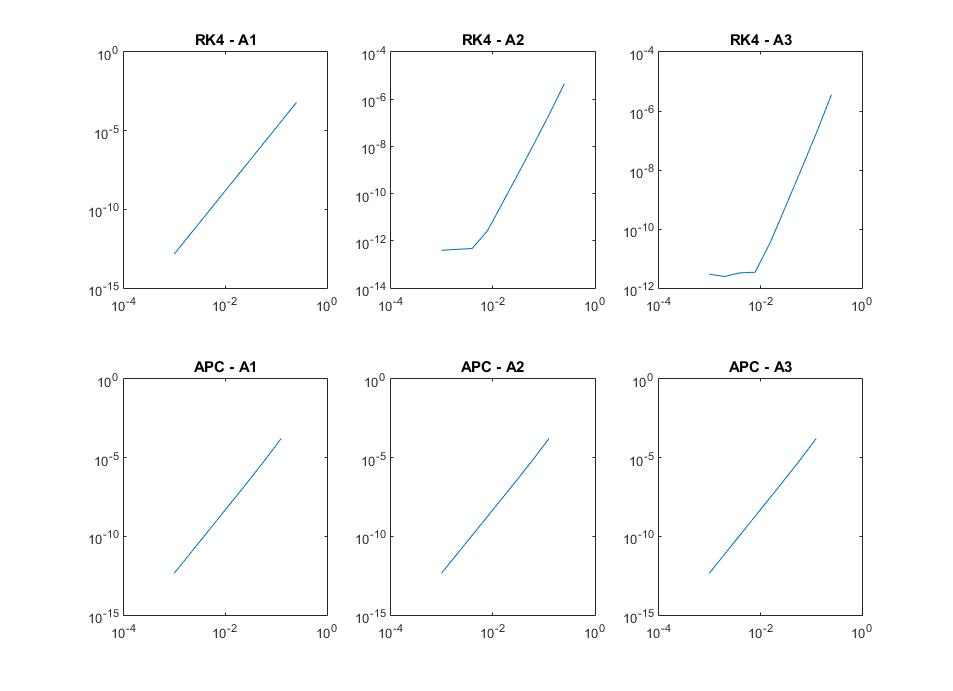
\includegraphics[scale=.6]{Plots}
\end{center}
The infinite values at step-size $h = \{1, 0.5\}$ were removed to correct the graphs. We see that the error for RK4 plateaus for A2 and A3, but Adams 4th Order Predictor-Corrector have a very linear log plot. The slopes are listed in the table below:
\begin{multicols}{2}
\begin{center}
\begin{tabular}{|c|c|}
\hline
Method/Test & Log Slope \\
\hline
RK4 - A1 & 3.9998 \\
\hline
RK4 - A2 & 3.1299 \\
\hline
RK4 - A3 & 2.6615 \\
\hline
\end{tabular}
\end{center}
\columnbreak
\begin{center}
\begin{tabular}{|c|c|}
\hline
Method/Test & Log Slope \\
\hline
APC - A1 & 4.0468 \\
\hline
APC - A2 & 4.0468 \\
\hline
APC - A2 & 4.0468 \\
\hline
\end{tabular}
\end{center}
\end{multicols}
We can note that the plateaus in RK4 - A2, A3 causes the fitted slope to be much lower than RK4 - A1. Similary, Adams 4th Order Predictor-Corrector have an extremely similar slope for all three cases.

\section{Discussion/Summary}
We can use the derived slopes in this case to determine the order of these two methods. Now we that are graphs described above are the logarithmic graphs of the error of our methods. In other words,
\begin{align} \nonumber
log(err(h)) &= m(log(h)) + b, \mbox{where } m \mbox{ is the slope} \\ \nonumber
&= log(h^m) + b \\ \nonumber
\\ \nonumber &\mbox{Take the power of e on both sides.} \\ \nonumber \\ \nonumber
err(h) &= e^{log(h^m) + b} \\ \nonumber
&= e^bh^m \\ \nonumber
\\ \nonumber &\mbox{Now note that for our linear plots, their slopes ~ 4, thus:} \\ \nonumber \\ \nonumber
err(h) &= e^bh^4 \\ \nonumber
&= O(h^4)
\end{align}
Thus, our methods RK4 and Adams 4th Order Predictor-Corrector are 4th order.
\end{document}